\documentclass[11pt]{standalone}
\usepackage{amssymb}
\usepackage{amsmath}
\usepackage[no-math]{fontspec}
\usepackage{unicode-math}
\setmainfont{Libertinus Sans}
\setsansfont{Libertinus Sans}
\setmathfont{Libertinus Math}
\usepackage{pgf,xcolor}
\usepackage{tikz}
\usetikzlibrary{arrows.meta, backgrounds, calc}
\usepackage{pgfplots}
\pgfplotsset{compat=newest}
\usepackage{pifont}

\definecolor{my_darkgray}{HTML}{484949}
\definecolor{my_lightgray}{HTML}{F3F4F4}
\definecolor{my_darkblue}{HTML}{005A94}
\definecolor{my_lightblue}{HTML}{CCDEE9}
\definecolor{my_yellow}{HTML}{FFEC7F}
\definecolor{my_red}{HTML}{E60000}
\definecolor{my_orange}{HTML}{E87846}

\begin{document}
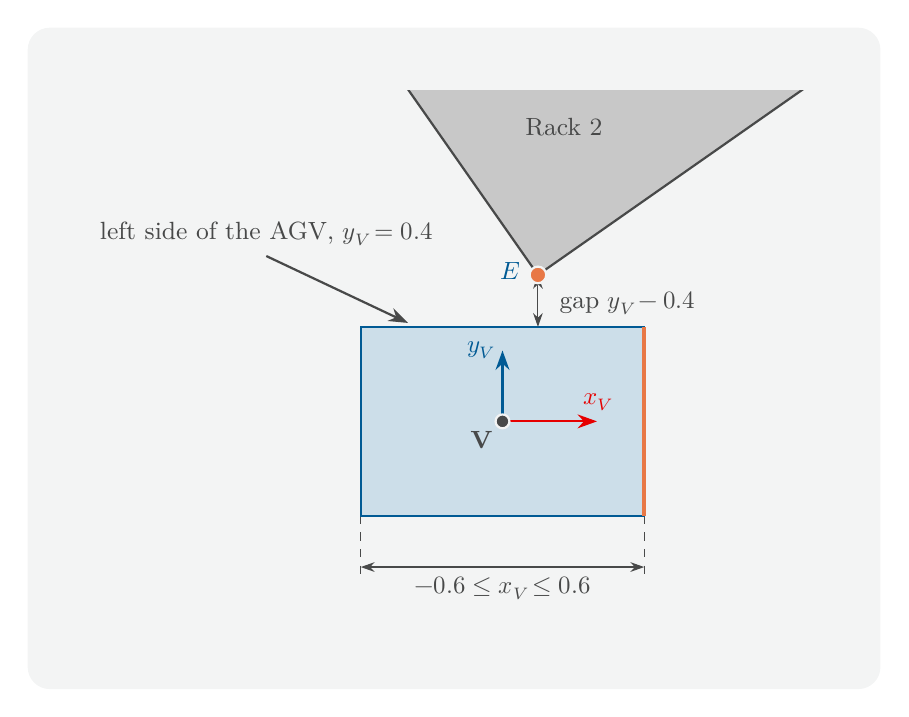
\begin{tikzpicture}[
    show background rectangle,
    background rectangle/.style={fill=my_lightgray, rounded corners=8pt},
    inner frame sep=0.8cm,
    achse/.style={thick, -{Stealth[length=7pt, width=5pt]}},
    bemassung/.style={draw=my_darkgray, thin, {Stealth[length=5pt, width=3.5pt]}-{Stealth[length=5pt, width=3.5pt]}},
    hilfslinie/.style={draw=my_darkgray, thin, dashed},
    annotation/.style={draw=my_darkgray, thick, -{Stealth[length=7pt, width=5pt]}}
]

    % FTF und Regalecke im Fahrzeugkoordinatensystem, Maßstab 1 m = 3 cm.
    % Fahrzeug 1.2 m x 0.8 m. Die Ecke E liegt schematisch bei (0.15, 0.62),
    % das Regal ist wie bei einem Gierwinkel von etwa 55 Grad gedreht: Seine
    % Kanten zeigen von E aus in die Richtungen 35 und 125 Grad.
    \coordinate (E) at (0.45,1.86);

    % Regal 2, in Fahrzeugkoordinaten schräg; es reicht über den Ausschnitt
    % hinaus, deshalb wird es am Bildrand abgeschnitten
    \begin{scope}
        \clip (-4.6,-2.6) rectangle (4.0,4.2);
        \fill[my_darkgray!30] (E) -- ($(E)+(125:5)$) -- ($(E)+(125:5)+(35:5)$)
            -- ($(E)+(35:5)$) -- cycle;
        \draw[draw=my_darkgray, thick] ($(E)+(125:5)$) -- (E) -- ($(E)+(35:5)$);
    \end{scope}
    \node[font=\small, text=my_darkgray] at ($(E)+(80:1.9)$) {Rack 2};

    % Streifen neben dem Fahrzeug: -0.6 <= x_V <= 0.6
    \draw[hilfslinie] (-1.8,-1.2) -- (-1.8,-2.0);
    \draw[hilfslinie] (1.8,-1.2) -- (1.8,-2.0);
    \draw[bemassung] (-1.8,-1.85) -- (1.8,-1.85)
        node[midway, anchor=north, font=\small, text=my_darkgray] {$-0.6 \leq x_V \leq 0.6$};

    % Fahrzeug: Umriss hellblau, Vorderkante orange
    \draw[fill=my_lightblue, draw=my_darkblue, thick] (-1.8,-1.2) rectangle (1.8,1.2);
    \draw[draw=my_orange, ultra thick] (1.8,-1.2) -- (1.8,1.2);

    % Fahrzeugkoordinatensystem F
    \coordinate (F) at (0,0);
    \draw[achse, draw=my_red] (F) -- (1.2,0)
        node[anchor=south, font=\small, text=my_red] {$x_V$};
    \draw[achse, draw=my_darkblue] (F) -- (0,0.9)
        node[anchor=east, font=\small, text=my_darkblue] {$y_V$};
    \node[font=\small\bfseries, text=my_darkgray, anchor=north east] at (F) {V};
    \draw[fill=my_darkgray, draw=my_lightgray, thick] (F) circle (2.5pt);

    % Linke Fahrzeugseite bei y_V = 0.4
    \draw[annotation] (-3.0,2.1) -- (-1.2,1.25);
    \node[font=\small, text=my_darkgray, anchor=south] at (-3.0,2.1)
        {left side of the AGV, $y_V = 0.4$};

    % Lücke zwischen linker Fahrzeugseite und Regalecke
    \draw[bemassung] (0.45,1.2) -- (E);
    \node[font=\small, text=my_darkgray, anchor=west] at (0.6,1.5) {gap $y_V - 0.4$};

    % Regalecke
    \draw[fill=my_orange, draw=my_lightgray, thick] (E) circle (3pt);
    \node[font=\small, text=my_darkblue, anchor=east] at ($(E)+(-0.12,0.05)$) {$E$};

\end{tikzpicture}
\end{document}
